\chapter{Sorting}

\section{Heap Sort}

\begin{minipage}[t]{0.45\linewidth}
    Implementation 1:

    \listu {
        \item Run \textsc{Build-Max-Heap}$(A)$
        \item Run \textsc{Extract-Max}$(A)$ for $n - 1$ times
    }
\end{minipage}
\begin{minipage}[t]{0.45\linewidth}
    Implementation 2:

    \listu {
        \item We modify the \textsc{Extract-Max} algorithm to swap the root with the last item
    }
\end{minipage}

\section{Quick Sort}

\begin{algorithm}[H] \begin{algorithmic}[1]
    \Procedure{QuickSort}{$A$}
        \If $\textsc{Len}(A) \le 1$ 
            \State \Return $A$
        \EndIf
        \State $L, p, G \gets \textsc{Partition}(A)$
        \State \Return $\textsc{QuickSort}(L) + [p] + \textsc{QuickSort}(G)$
    \EndProcedure
\end{algorithmic} \end{algorithm}

\subsection{Deterministic Quick Sort}

In deterministic quick sort, we choose the pivot to be a certain index in the array. We can choose the pivot to be the first element, the last element, or the middle element. 

\listu {
    \item Run-time depends on input ordering
    \item Bad ordering would yield bad run-time, while random ordering would generally yield better run-time
}

\subsection{Randomized Quick Sort}

In randomized quick sort, we choose the pivot to be a random index in the array. Intuitively, the expected run-time would be the same as deterministic quick sort -- $\Theta(n \lg n)$ -- but the worst case run-time would be much better.

\section{Topology Sort}

\example {
    We wish to determine the sequence of courses to take during our undergraduate program

    \listu {
        \item A university course $C$ may have a set of prerequisite courses that must be completed before $C$
        \item How can we determine a valid sequence of courses to take?
    }

    \begin{center} 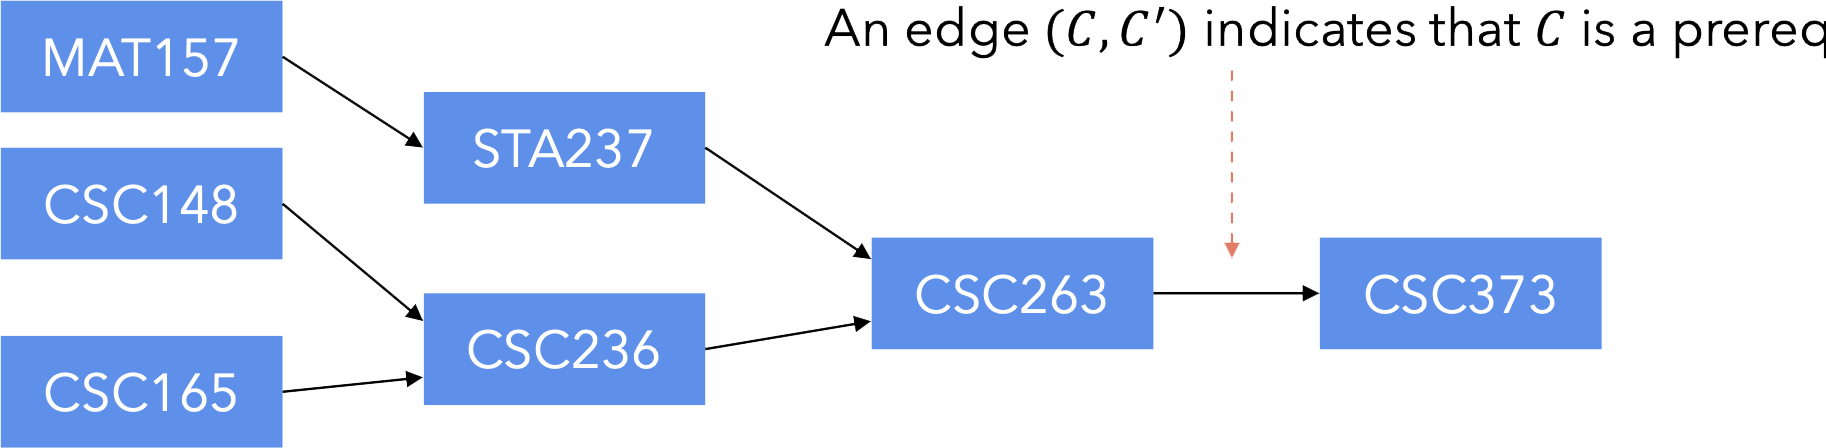
\includegraphics[width=0.5\linewidth]{images/Topology-Sorting-Example.png} \end{center}

    When we add more nodes/edges, things become less clear

    \begin{center} 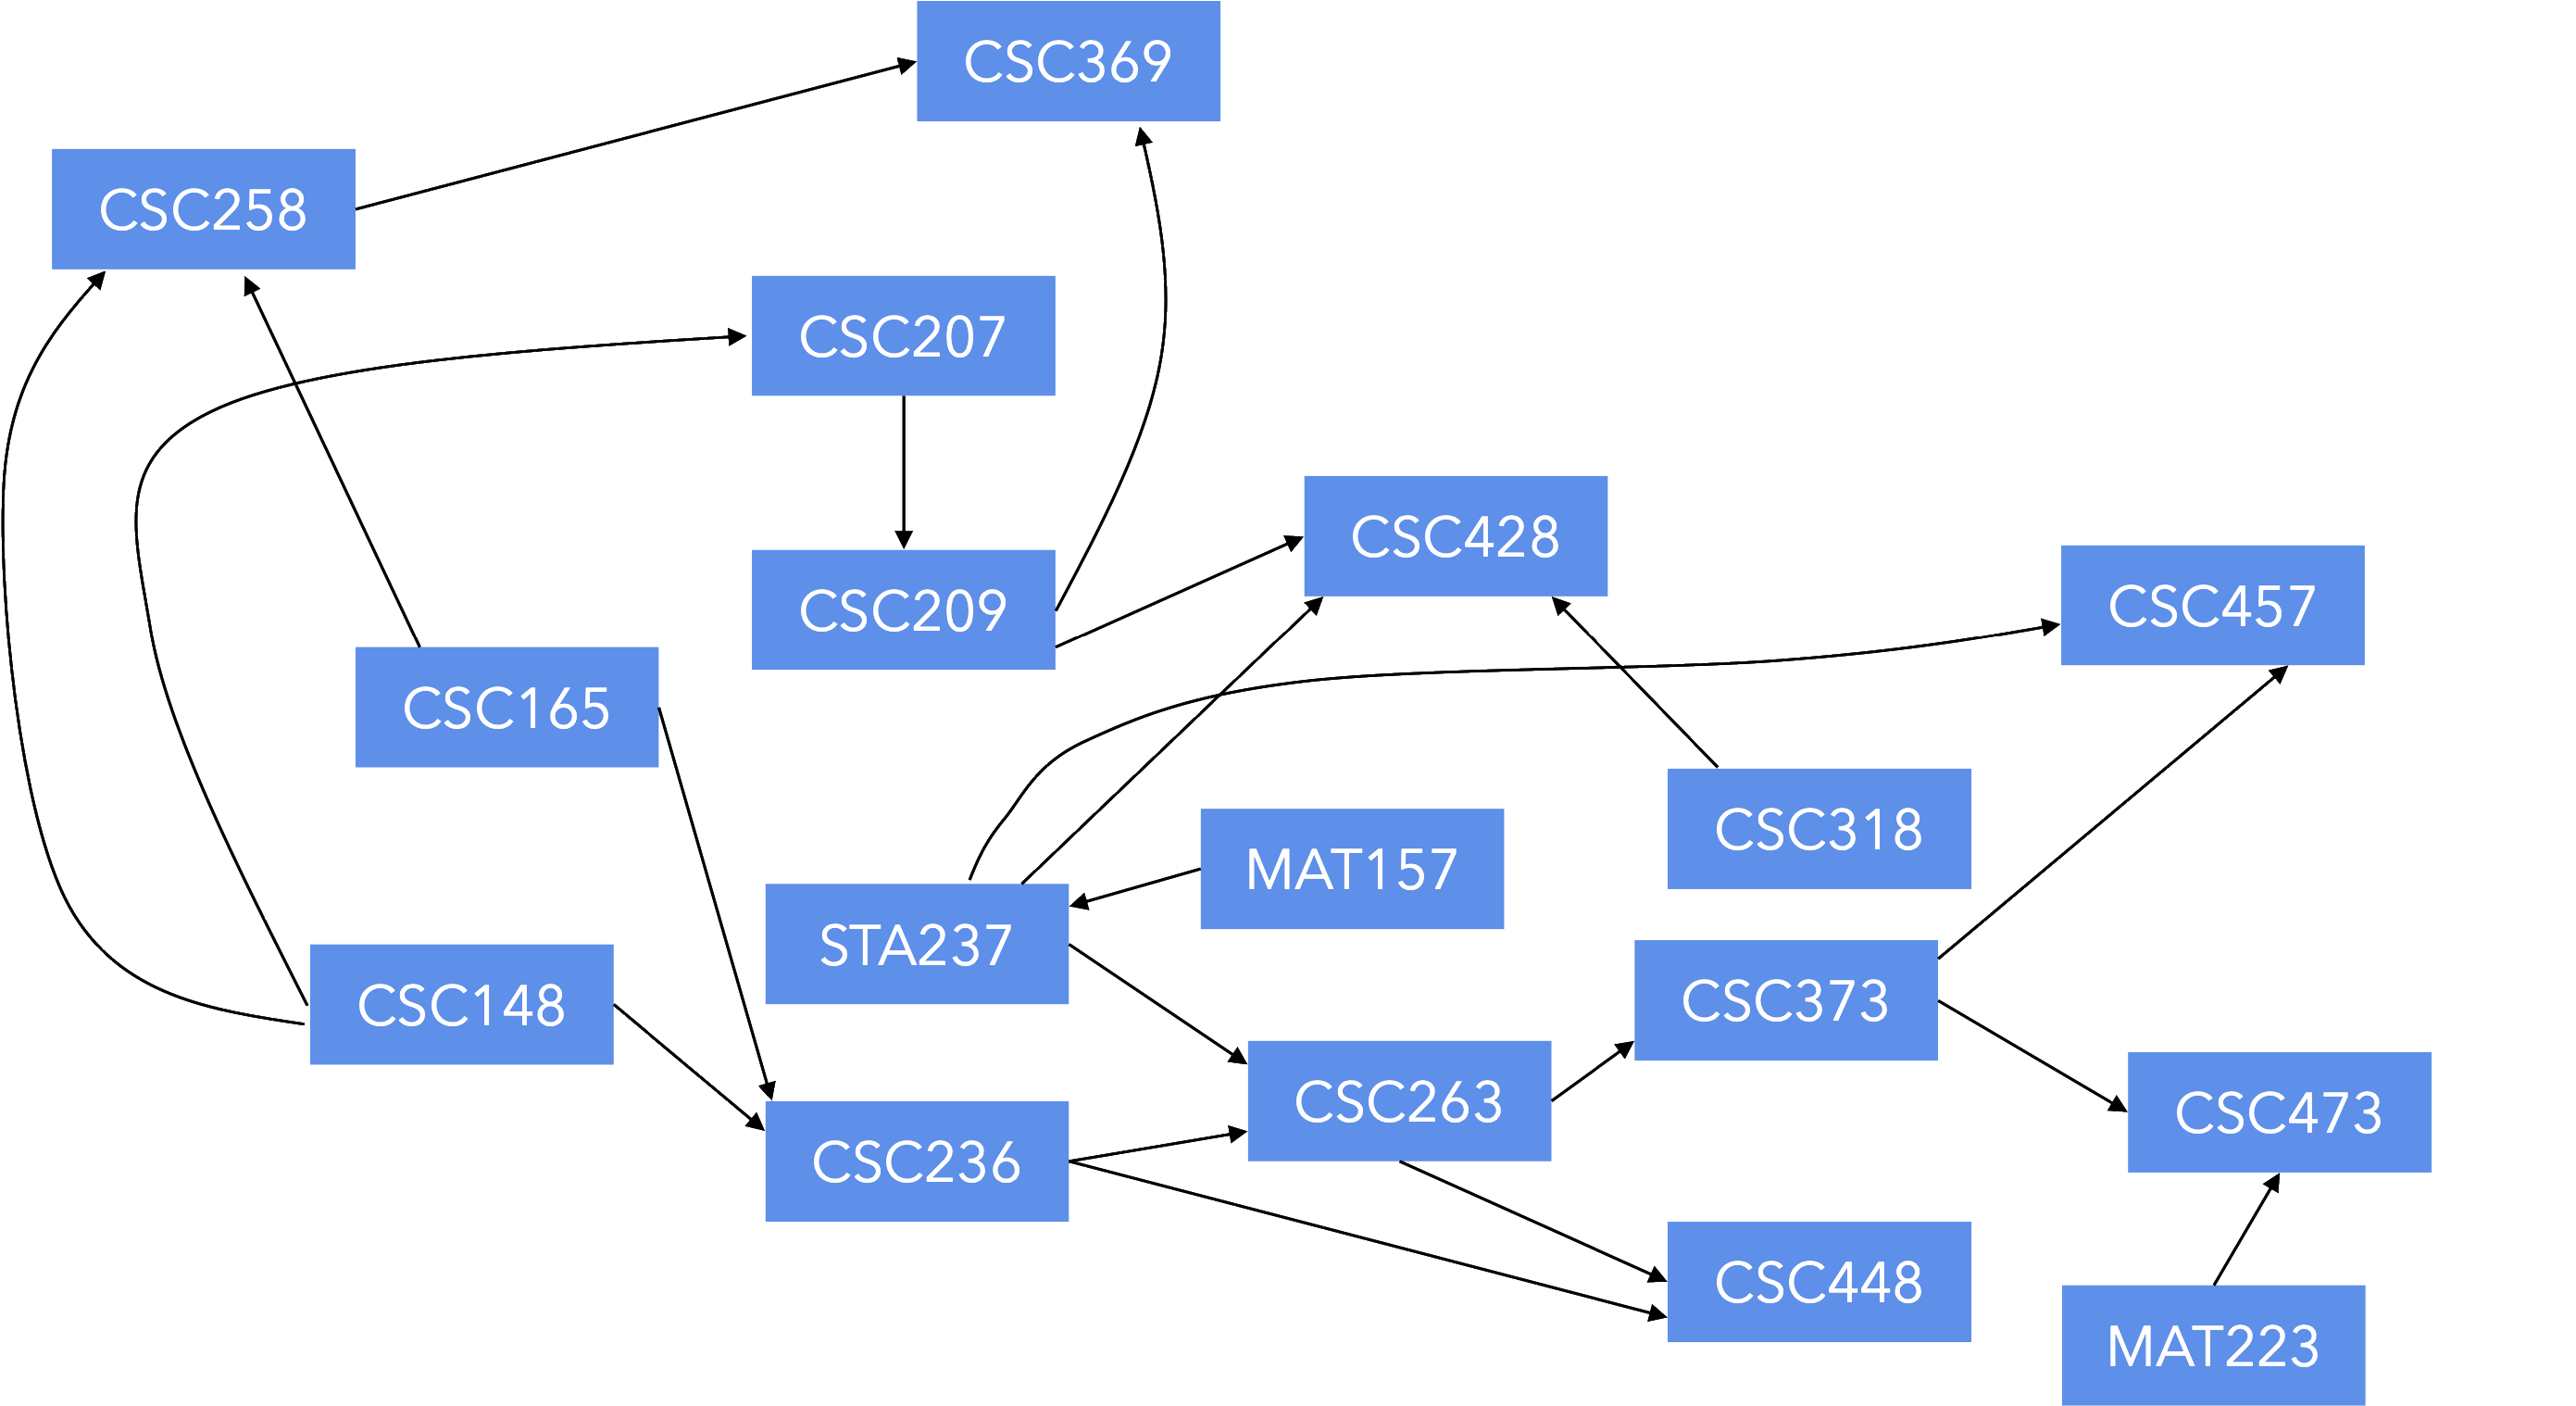
\includegraphics[width=0.75\linewidth]{images/Topology-Sorting-Example-Large.png} \end{center}
}

\subsection{Directed Acyclic Graphs}

A directed acyclic graph (or DAG) is a directed graph with no cycles

\begin{center} 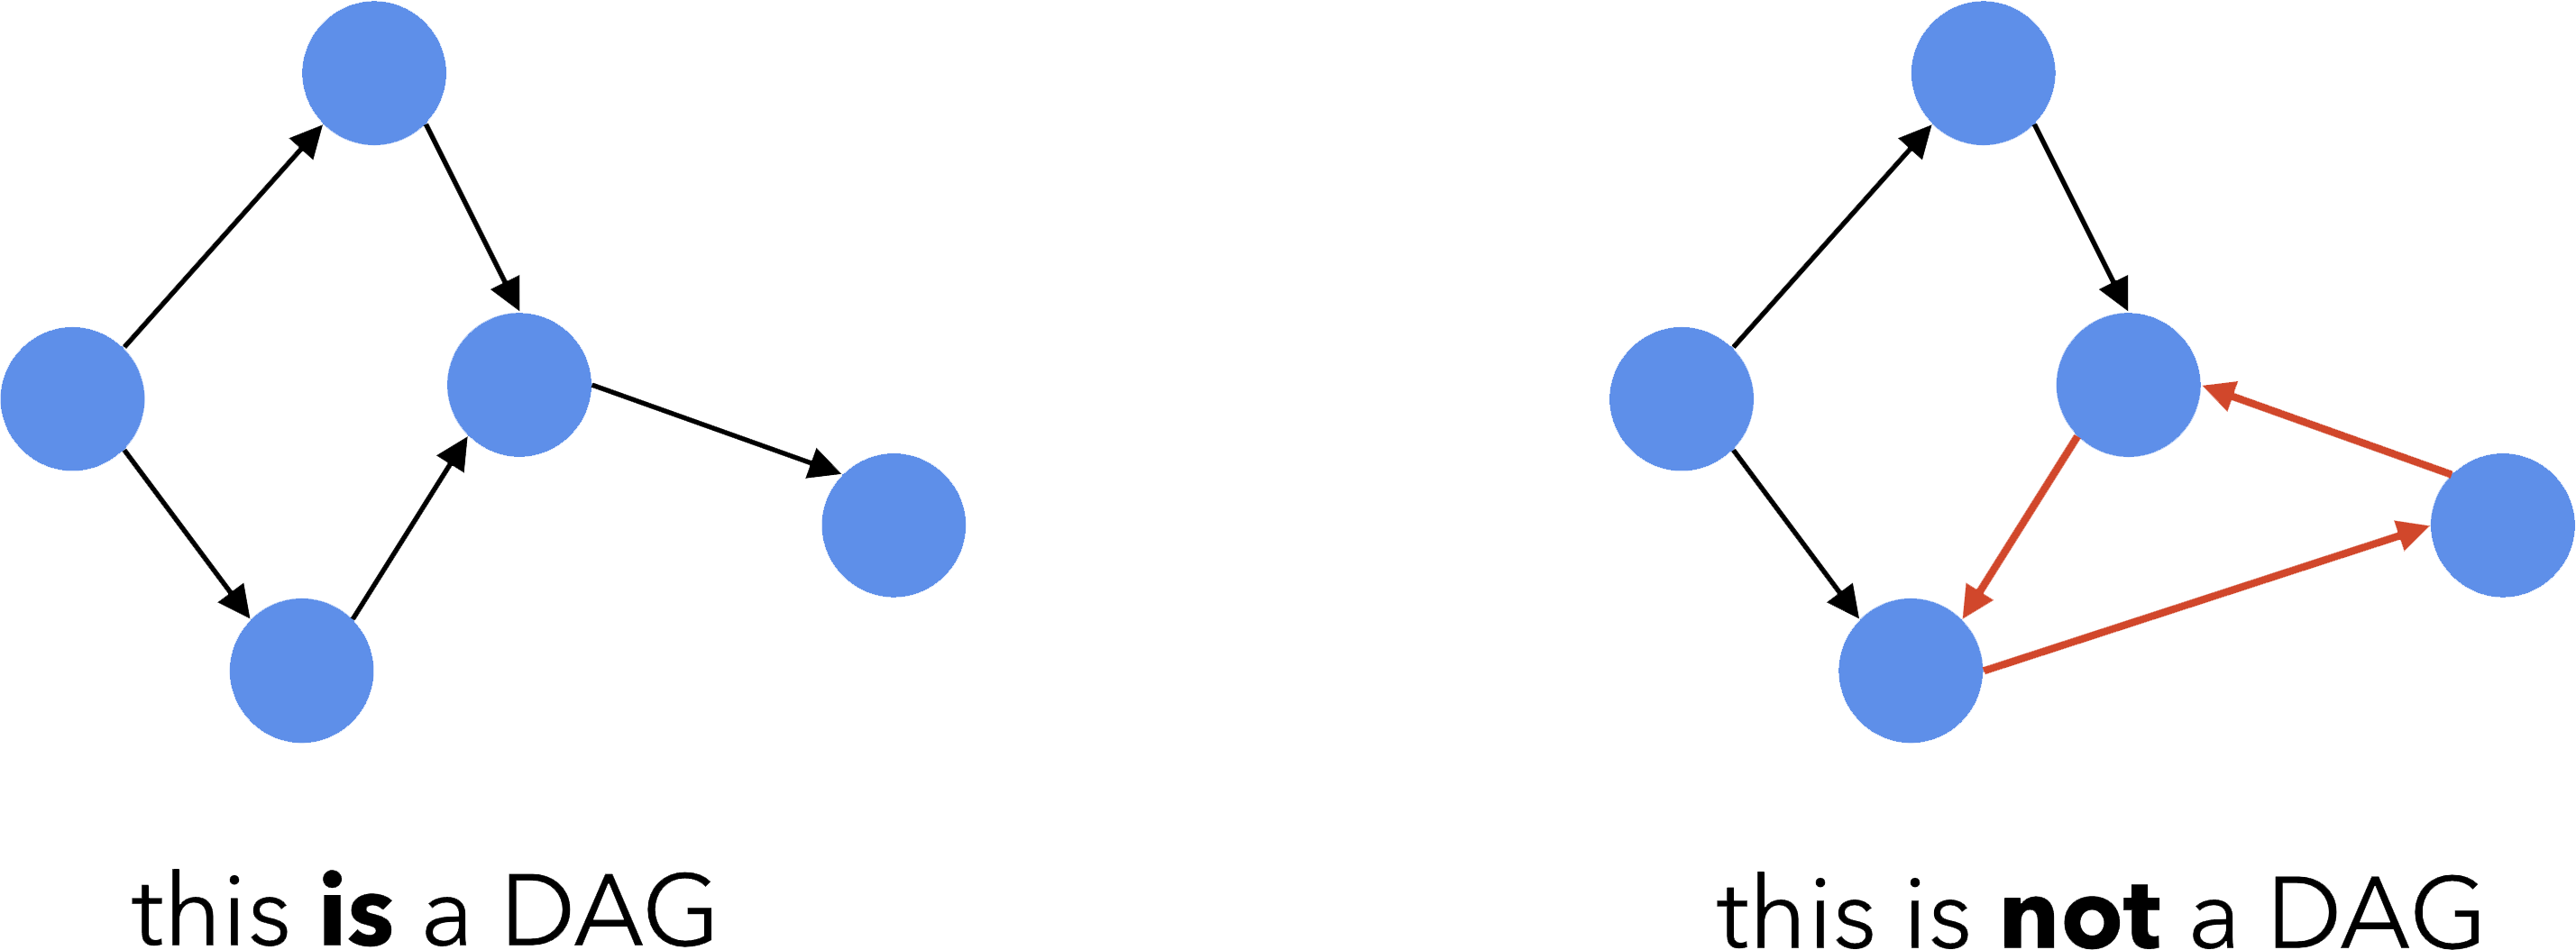
\includegraphics[width=0.45\linewidth]{images/DAG.png} \end{center}

\subsection{Topological Sort}

A topological sort/ordering of a DAG $G = (V, E)$ is a sequence of its vertices such that, if $(u, v) \in E$, then $u$ appears before $v$ in the sequence

\begin{center} 
    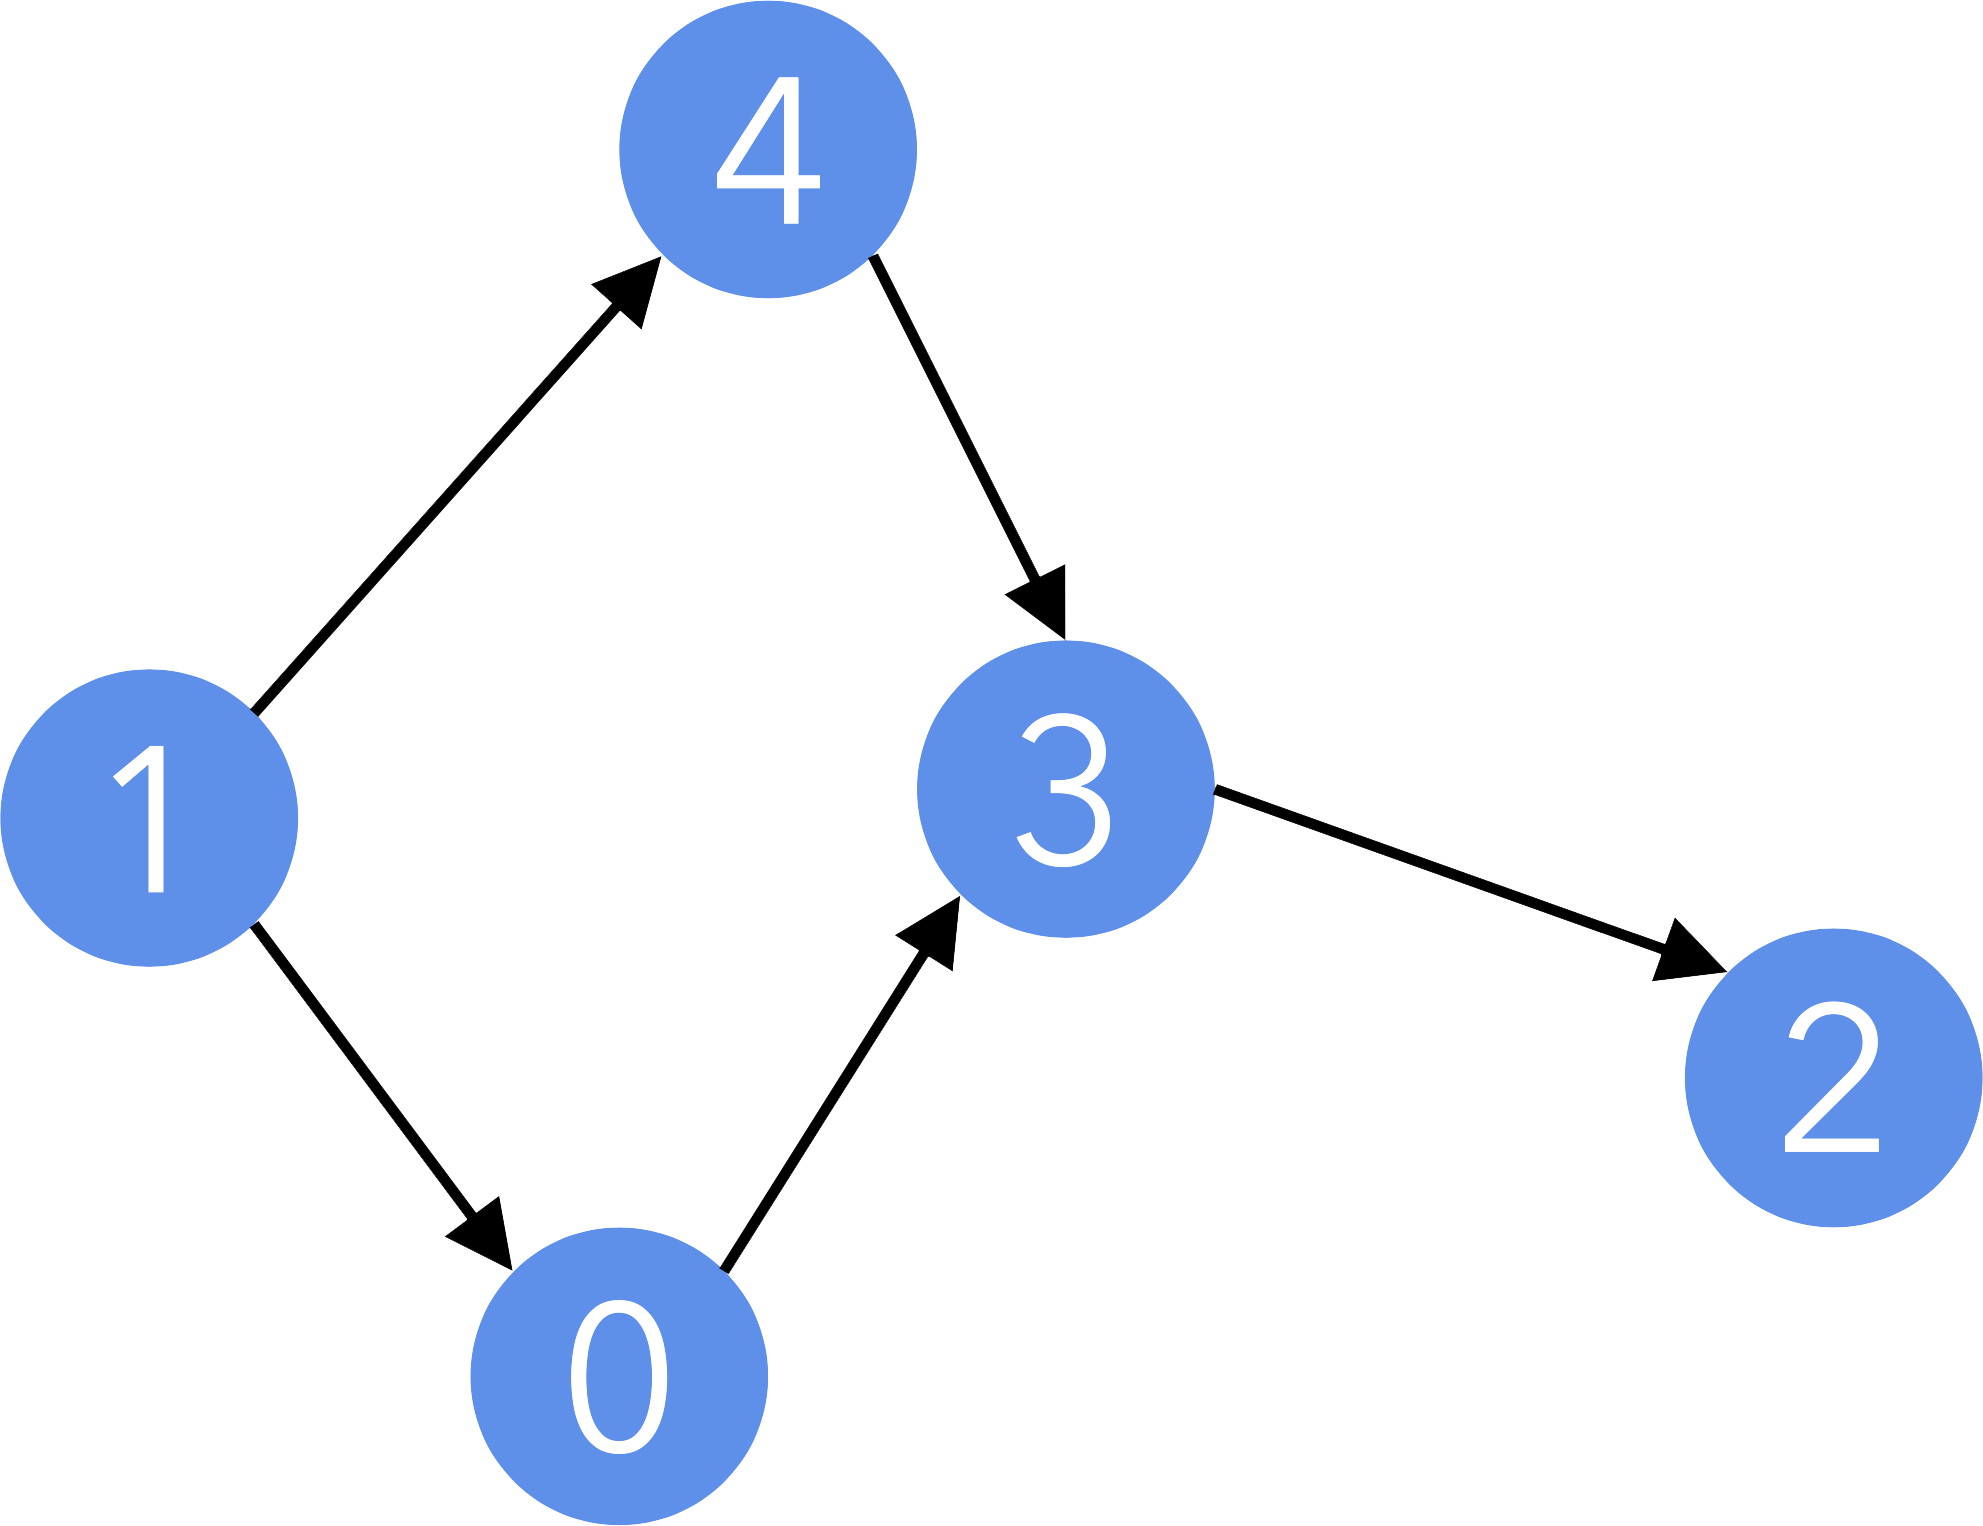
\includegraphics[width=0.2\linewidth]{images/Topological-Sorting.png} 

    1, 0, 4, 3, 2 is a topological ordering of these vertices
\end{center}

Given a DAG $G = (V, E)$, how can we efficiently compute a topological ordering of $G$?

\listu {
    \item Claim: if we perform DFS on a DAG $G$, the resulting DFS forest contains no back edges.
    \item Claim: every out-neighbour of every vertex $v$ has an earlier `visited' time than $v$.
    
    \listu {
        \item If $(v, u)$ is a tree / forward edge, then $u$ is a descendant of $v$. By the Parenthesis Theorem, $\left[ \textit{disc}[u] , \textit{vis}[u] \right]$ is contained in $\left[ \textit{disc}[v], \textit{vis}[v] \right]$. Hence, $\textit{vis}[u] < \textit{vis}[v]$.
        \item If $(v, u)$ is a cross edge, then $u$ was already visited by the time we finish visiting $v$. Hence, $\textit{vis}[u] < \textit{vis}[v]$.
    }
}

We claim that a directed graph $G$ can be topologically sorted iff $G$ contains no cycles iff \textsc{DFS} finds no back edges. 

\listo {
    \item Maintain a linked list $L$ while performing \textsc{DFS} on $G = (V, E)$
    \item When we finish visiting a node $v$ (by setting $\textit{vis}[v]$ and painting $v$ black), add $v$ to the head of the linked list $L$
    \item Once DFS terminates, $L$ contains a list of all vertices in $V$ sorted in decreasing order by their `visited' times
}